\chapter{Introduction to Optimization}
Linear Programming is a sub-field of optimization theory, which is itself a sub-field of Applied Mathematics. Applied Mathematics is a very general area of study that could arguably encompass half of the engineering disciplines--if you feel like getting into an argument with an engineer. Put simply, applied mathematics is all about applying mathematical techniques to understand or do something practical. 

Optimization is an exciting sub-discipline within applied mathematics! Optimization is all about making things better; this could mean helping a company make better decisions to maximize profit; helping a factory make products with less environmental impact; or helping a zoologist improve the diet of an animal. When we talk about optimization, we often use terms like \textit{better} or \textit{improvement}. It's important to remember that words like better can mean \textit{more of something} (as in the case of profit) or \textit{less of something} as in the case of waste. As we study linear programming, we'll quantify these terms in a mathematically precise way. For the time being, let's agree that when we optimize something we are trying to make some decisions that will make it better.

\begin{example}
Let's recall a simple optimization problem from differential calculus (Math 140): Goats are an environmentally friendly and inexpensive way to control a lawn when there are lots of rocks or lots of hills. (Seriously, both Google and some U.S. Navy bases use goats on rocky hills instead of paying lawn mowers!) 

Suppose I wish to build a pen to keep some goats. I have 100 meters of fencing and I wish to build the pen in a rectangle with the largest possible area. How long should the sides of the rectangle be? In this case, making the pen \textit{better} means making it have the largest possible area.

The problem is illustrated in Figure \ref{fig:GoatPen}.
\begin{figure}[htbp]
\centering
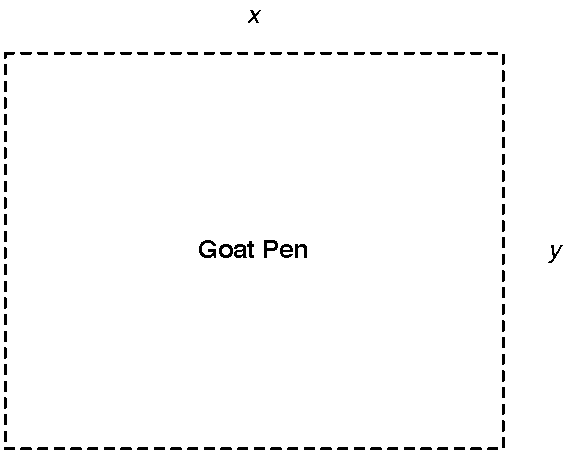
\includegraphics[scale=0.6]{GoatPen.pdf}
\caption{Goat pen with unknown side lengths. The objective is to identify the values of $x$ and $y$ that maximize the area of the pen (and thus the number of goats that can be kept).}
\label{fig:GoatPen}
\end{figure}
Clearly, we know that:
\begin{equation}
2x + 2y = 100
\label{eqn:GoatPerimeter}
\end{equation}
because $2x + 2y$ is the perimeter of the pen and I have 100 meters of fencing to build my pen. The area of the pen is $A(x,y) = xy$. We can use Equation \ref{eqn:GoatPerimeter} to solve for $x$ in terms of $y$. Thus we have:
\begin{equation}
y = 50 - x
\end{equation}
and $A(x) = x(50-x)$. To maximize $A(x)$, recall we take the first derivative of $A(x)$ with respect to $x$, set this derivative to zero and solve for $x$:
\begin{equation}
\frac{dA}{dx} = 50-2x = 0;
\end{equation}
Thus, $x = 25$ and $y = 50-x = 25$. We further recall from basic calculus how to confirm that this is a maximum; note:
\begin{equation}
\left.\frac{d^2A}{dx^2}\right|_{x = 25} = -2 < 0
\end{equation}
Which implies that $x = 25$ is a \textit{local maximum} for this function. Another way of seeing this is to note that $A(x) = 50x-x^2$ is an ``upside-down'' parabola. As we could have guessed, a square will maximize the area available for holding goats. 
\label{ex:GoatExample}
\end{example}

\begin{exercise} A canning company is producing canned corn for the holidays. They have determined that each family prefers to purchase their corn in units of 12 fluid ounces. Assuming that metal costs 1 cent per square inch and 1 fluid ounce is about 1.8 cubic inches, compute the ideal height and radius for a can of corn assuming that cost is to be minimized. [Hint: Suppose that our can has radius $r$ and height $h$. The formula for the surface area of a can is $2\pi r h + 2 \pi r^2$. Since metal is priced by the square inch, the cost is a function of the surface area. The volume of the can is $\pi r ^2 h$ and is constrained. Use the same trick we did in the example to find the values of $r$ and $h$ that minimize cost.
\label{exer:Can}
\end{exercise}

\section{A General Maximization Formulation}
Let's take a more general look at the goat pen example. The area function is a mapping from $\mathbb{R}^2$ to $\mathbb{R}$, written $A : \mathbb{R}^2 \rightarrow \mathbb{R}$. The domain of $A$ is the two dimensional space $\mathbb{R}^2$ and its range is $\mathbb{R}$.

Our objective in Example \ref{ex:GoatExample} is to maximize the function $A$ by choosing values for $x$ and $y$. In optimization theory, the function we are trying to maximize (or minimize) is called the \textit{objective function}. In general, an objective function is a mapping $z: D \subseteq \mathbb{R}^n \rightarrow \mathbb{R}$. Here $D$ is the domain of the function $z$. 

\begin{definition} Let $z: D \subseteq \mathbb{R}^n \rightarrow \mathbb{R}$. The point $\mathbf{x}^*$ is a \textit{global maximum} for $z$ if for all $\mathbf{x} \in D$, $z(\mathbf{x}^*) \geq z(\mathbf{x})$. 
A point $\mathbf{x}^* \in D$ is a \textit{local maximum} for $z$ if there is a neighborhood $S \subseteq D$ of  $\mathbf{x}^*$  (i.e., $\mathbf{x}^* \in S$) so that for all $\mathbf{x} \in S$, $z(\mathbf{x}^*) \geq z(\mathbf{x})$. 
\label{defn:Max}
\end{definition}

\begin{remark} Clearly Definition \ref{defn:Max} is valid only for domains and functions where the concept of a neighborhood is defined and understood. In general, $S$ must be a topologically connected set (as it is in a neighborhood in $\mathbb{R}^n$) in order for this definition to be used or at least we must be able to define the concept of \textit{neighborhood} on the set\footnote{Thanks to Bob Pakzad-Hurson who suggested this remark for versions after 1.1.}.
\end{remark}

\begin{exercise} Using analogous reasoning write a definition for a global and local minimum. [Hint: Think about what a minimum means and find the correct direction for the $\geq$ sign in the definition above.]
\end{exercise}

In Example \ref{ex:GoatExample}, we are constrained in our choice of $x$ and $y$ by the fact that $2x + 2y = 100$. This is called a \textit{constraint} of the optimization problem. More specifically, it's called an \textit{equality constraint}. If we did not need to use all the fencing, then we could write the constraint as $2x + 2y \leq 100$, which is called an \textit{inequality constraint}. In complex optimization problems, we can have many constraints. The set of all points in $\mathbb{R}^n$ for which the constraints are true is called the \textit{feasible set} (or feasible region). Our problem is to \textit{decide} the best values of $x$ and $y$ to maximize the area $A(x,y)$. The variables $x$ and $y$ are called \textit{decision variables}. 

Let $z:D\subseteq\mathbb{R}^n \rightarrow \mathbb{R}$; for $i=1,\dots,m$, $g_i:D\subseteq\mathbb{R}^n \rightarrow \mathbb{R}$; and for $j=1,\dots,l$ $h_j:D\subseteq\mathbb{R}^n \rightarrow \mathbb{R}$ be functions. Then the general maximization problem with objective function $z(x_1,\dots,x_n)$ and \textit{inequality constraints} $g_i(x_1,\dots,x_n) \leq b_i$ ($i=1,\dots,m$) and \textit{equality constraints} $h_j(x_1,\dots,x_n) = r_j$ is written as:
\begin{equation}
\left\{
\begin{aligned}
\max\;\;& z(x_1,\dots,x_n)\\
s.t.\;\;& g_1(x_1,\dots,x_n) \leq b_1\\
& \hspace*{0.5in}\vdots\\
& g_m(x_1,\dots,x_n) \leq b_m\\
& h_1(x_1,\dots,x_n) = r_1\\
&\hspace*{0.5in}\vdots\\
&h_l(x_1,\dots,x_n) = r_l
\end{aligned}
\right.
\label{eqn:GeneralMax}
\end{equation}
Expression \ref{eqn:GeneralMax} is also called a \textit{mathematical programming problem}. Naturally when constraints are involved we define the global and local maxima for the objective function $z(x_1,\dots,x_n)$ in terms of the feasible region instead of the entire domain of $z$, since we are only concerned with values of $x_1,\dots,x_n$ that satisfy our constraints.

\begin{example}[Continuation of Example \ref{ex:GoatExample}] We can re-write the problem in Example \ref{ex:GoatExample}:
\begin{equation}
\left\{
\begin{aligned}
\max \;\; & A(x,y) = x y \\
s.t. \;\; & 2x + 2y = 100\\
& x \geq 0\\
& y \geq 0 
\end{aligned}\right.
\label{eqn:GoatMax}
\end{equation}
Note we've added two inequality constraints $x \geq 0$ and $y \geq 0$ because it doesn't really make any sense to have negative lengths. We can re-write these constraints as $-x \leq 0$ and $-y \leq 0$ where $g_1(x,y) = -x$ and $g_2(x,y) = -y$ to make Expression \ref{eqn:GoatMax} look like Expression \ref{eqn:GeneralMax}.
\end{example}

We have formulated the general \textit{maximization} problem in Proble \ref{eqn:GeneralMax}. Suppose that we are interested in finding a value that minimizes an objective function $z(x_1,\dots,x_n)$ subject to certain constraints. Then we can write Problem \ref{eqn:GeneralMax} replacing $\max$ with $\min$. 

\begin{exercise} Write the problem from Exercise \ref{exer:Can} as a general minimization problem. Add any appropriate non-negativity constraints. [Hint: You must change $\max$ to $\min$.] 
\end{exercise}

An alternative way of dealing with minimization is to transform a minimization problem into a maximization problem. If we want to minimize $z(x_1,\dots,x_n)$, we can maximize $-z(x_1,\dots,x_n)$. In maximizing the negation of the objective function, we are actually finding a value that minimizes $z(x_1,\dots,x_n)$.

\begin{exercise} Prove the following statement:
\textit{Consider Problem \ref{eqn:GeneralMax} with the objective function $z(x_1,\dots,x_n)$ replaced by $-z(x_1,\dots,x_n)$. Then the solution to this new problem minimizes $z(x_1,\dots,x_n)$ subject to the constraints of Problem \ref{eqn:GeneralMax}.}[Hint: Use the definition of global maximum and a multiplication by $-1$. Be careful with the direction of the inequality when you multiply by $-1$.]
\label{exer:MinForMax}
\end{exercise}
%\begin{proof} Let $(x_1^*,\dots,x_n^*)$ maximize $-z(x_1,\dots,x_n)$ subject to the constraints of Problem \ref{eqn:GeneralMax}. Then for all other $(x_1,\dots,x_n)$ satisfying the constraints of Problem \ref{eqn:GeneralMax} we have: 
%\begin{displaymath}
%-z(x_1^*,\dots,x_n^*) \geq -z(x_1^*,\dots,x_n^*)
%\end{displaymath}
%Multiplying by $-1$ on both sides yields:
%\begin{displaymath}
%z(x_1^*,\dots,x_n^*) \leq z(x_1^*,\dots,x_n^*)
%\end{displaymath}
%and this holds for all other $(x_1,\dots,x_n)$ satisfying the constraints of Problem \ref{eqn:GeneralMax}. Thus $(x_1^*,\dots,x_n^*)$ is a solution to the problem of minimizing $z(x_1,\dots,x_n)$ subject to the constraints of Problem \ref{eqn:GeneralMax}. 
%\end{proof} 

\section{Some Geometry for Optimization}
A critical part of optimization theory is understanding the geometry of Euclidean space. To that end, we're going to review some critical concepts from Vector Calculus (Math 230/231). I'll assume that you remember some basic definitions like \textit{partial derivative} and \textit{Euclidean space}. If you need a refresher, you might want to consult \cite{MT03, Stew07}. 

We'll denote vectors in $\mathbb{R}^n$ in boldface. So $\mathbf{x} \in \mathbb{R}^n$ is an n-dimensional vector and we have $\mathbf{x} = (x_1,\dots,x_n)$. %It's common to associate an $n$-dimensional vectors with a $1 \times n$ matrix(row vector) or an $n \times 1$ matrix (column vector). 
\begin{definition}[Dot Product]
Recall that if $\mathbf{x}, \mathbf{y} \in \mathbb{R}^n$ are two $n$-dimensional vectors, then the \textit{dot product} (\textit{scalar product}) is:
\begin{equation}
\mathbf{x} \cdot \mathbf{y} = \sum_{i=1}^{n} x_i y_i
\end{equation}
where $x_i$ is the $i^\text{th}$ component of the vector $\mathbf{x}$. 
\end{definition}

An alternative and useful definition for the dot product is given by the following formula. Let $\theta$ be the angle between the vectors $\mathbf{x}$ and $\mathbf{y}$. Then the dot product of $\mathbf{x}$ and $\mathbf{y}$ may be alternatively written as:
\begin{equation}
\mathbf{x}\cdot\mathbf{y} = ||\mathbf{x}||||\mathbf{y}||\cos\theta
\end{equation}
This fact can be proved using the \textit{law of cosines} from trigonometry. As a result, we have the following small lemma (which is proved as Theorem 1 of \cite{MT03}):
\begin{lemma} Let $\mathbf{x}, \mathbf{y} \in \mathbb{R}^n$. Then the following hold:
\begin{enumerate*}
\item  The angle between $\mathbf{x}$ and $\mathbf{y}$ is less than $\pi/2$ (i.e., acute) iff $\mathbf{x}\cdot\mathbf{y} > 0$. 
\item The angle between $\mathbf{x}$ and $\mathbf{y}$ is exactly $\pi/2$ (i.e., the vectors are orthogonal) iff $\mathbf{x}\cdot\mathbf{y} = 0$. 
\item The angle between $\mathbf{x}$ and $\mathbf{y}$ is greater than $\pi/2$ (i.e., obtuse) iff $\mathbf{x}\cdot\mathbf{y} < 0$.
\end{enumerate*}
\end{lemma}

\begin{exercise} Use the value of the cosine function and the fact that $\mathbf{x}\cdot\mathbf{y} = ||\mathbf{x}||||\mathbf{y}||\cos\theta$ to prove the lemma. [Hint: For what values of $\theta$ is $\cos\theta > 0$.]
\end{exercise}

\begin{definition}[Graph] Let $z:D \subseteq \mathbb{R}^n \rightarrow \mathbb{R}$ be function, then the \textit{graph} of $z$ is the set of $n+1$ tuples:
\begin{equation}
\{(\mathbf{x},z(\mathbf{x})) \in \mathbb{R}^{n+1} | \mathbf{x} \in D\}
\end{equation}
\label{def:Graph}
\end{definition}
When $z: D \subseteq \mathbb{R} \rightarrow \mathbb{R}$, the graph is precisely what you'd expect. It's the set of pairs $(x,y) \in \mathbb{R}^2$ so that $y = z(x)$. This is the graph that you learned about back in Algebra 1.  

\begin{definition}[Level Set] Let $z:\mathbb{R}^n \rightarrow \mathbb{R}$ be a function and let $c \in \mathbb{R}$. Then the \textit{level set of value $c$ for function $z$} is the set:
\begin{equation}
\{\mathbf{x}=(x_1,\dots,x_n) \in \mathbb{R}^n | z(\mathbf{x}) = c\} \subseteq \mathbb{R}^n
\end{equation} 
\label{def:LevelSet}
\end{definition}

\begin{example} Consider the function $z = x^2 + y^2$. The level set of $z$ at $4$ is the set of points $(x,y) \in \mathbb{R}^2$ such that:
\begin{equation}
x^2 + y^2 = 4
\end{equation}
You will recognize this as the equation for a circle with radius 4. We illustrate this in the following two figures. Figure \ref{fig:LevelSet3D} shows the level sets of $z$ as they sit on the 3D plot of the function, while Figure \ref{fig:LevelSet2D} shows the level sets of $z$ in $\mathbb{R}^2$. The plot in Figure \ref{fig:LevelSet2D} is called a \textit{contour plot}. 
\begin{figure}[ht]
\centering
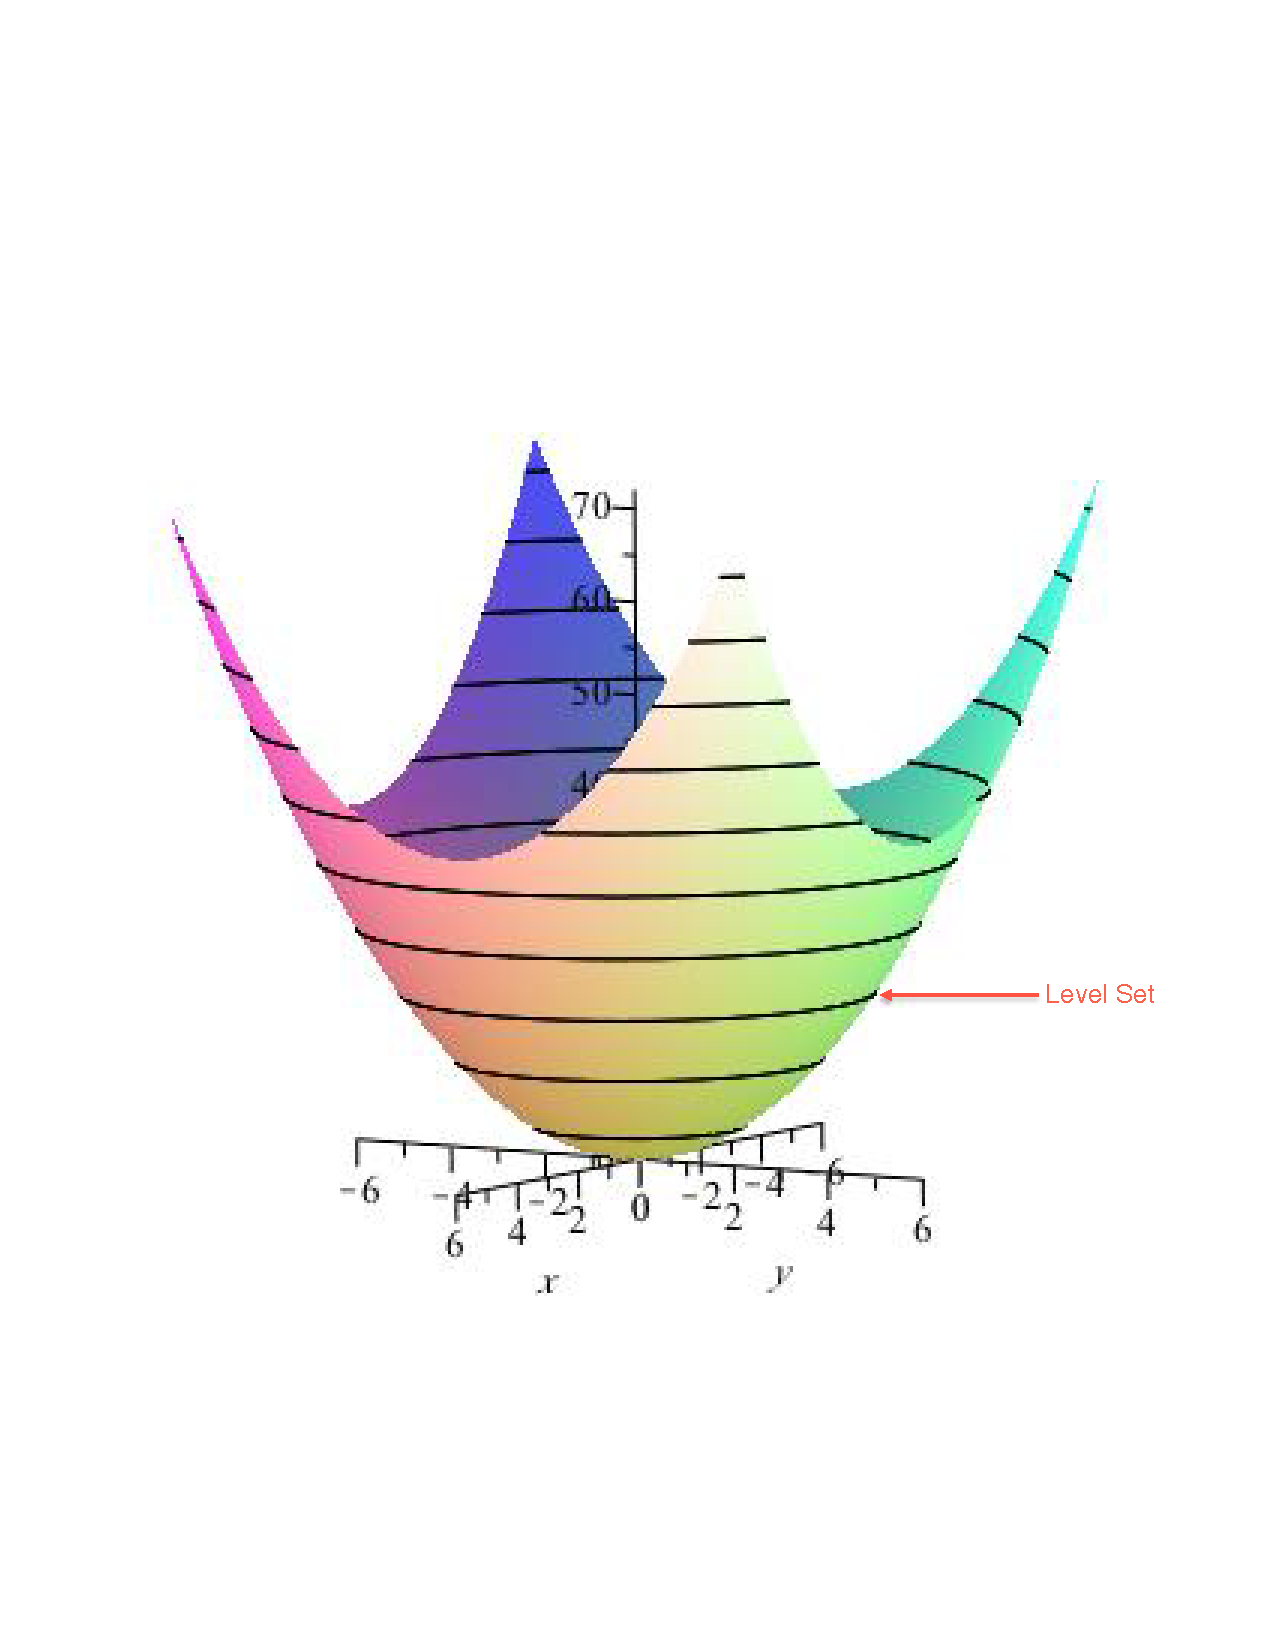
\includegraphics[scale=0.25]{LevelSetPlotNote.pdf}
\caption{Plot with Level Sets Projected on the Graph of $z$. The level sets existing in $\mathbb{R}^2$ while the graph of $z$ existing $\mathbb{R}^3$. The level sets have been projected onto their appropriate heights on the graph.}
\label{fig:LevelSet3D}
\end{figure}
\begin{figure}[ht]
\centering
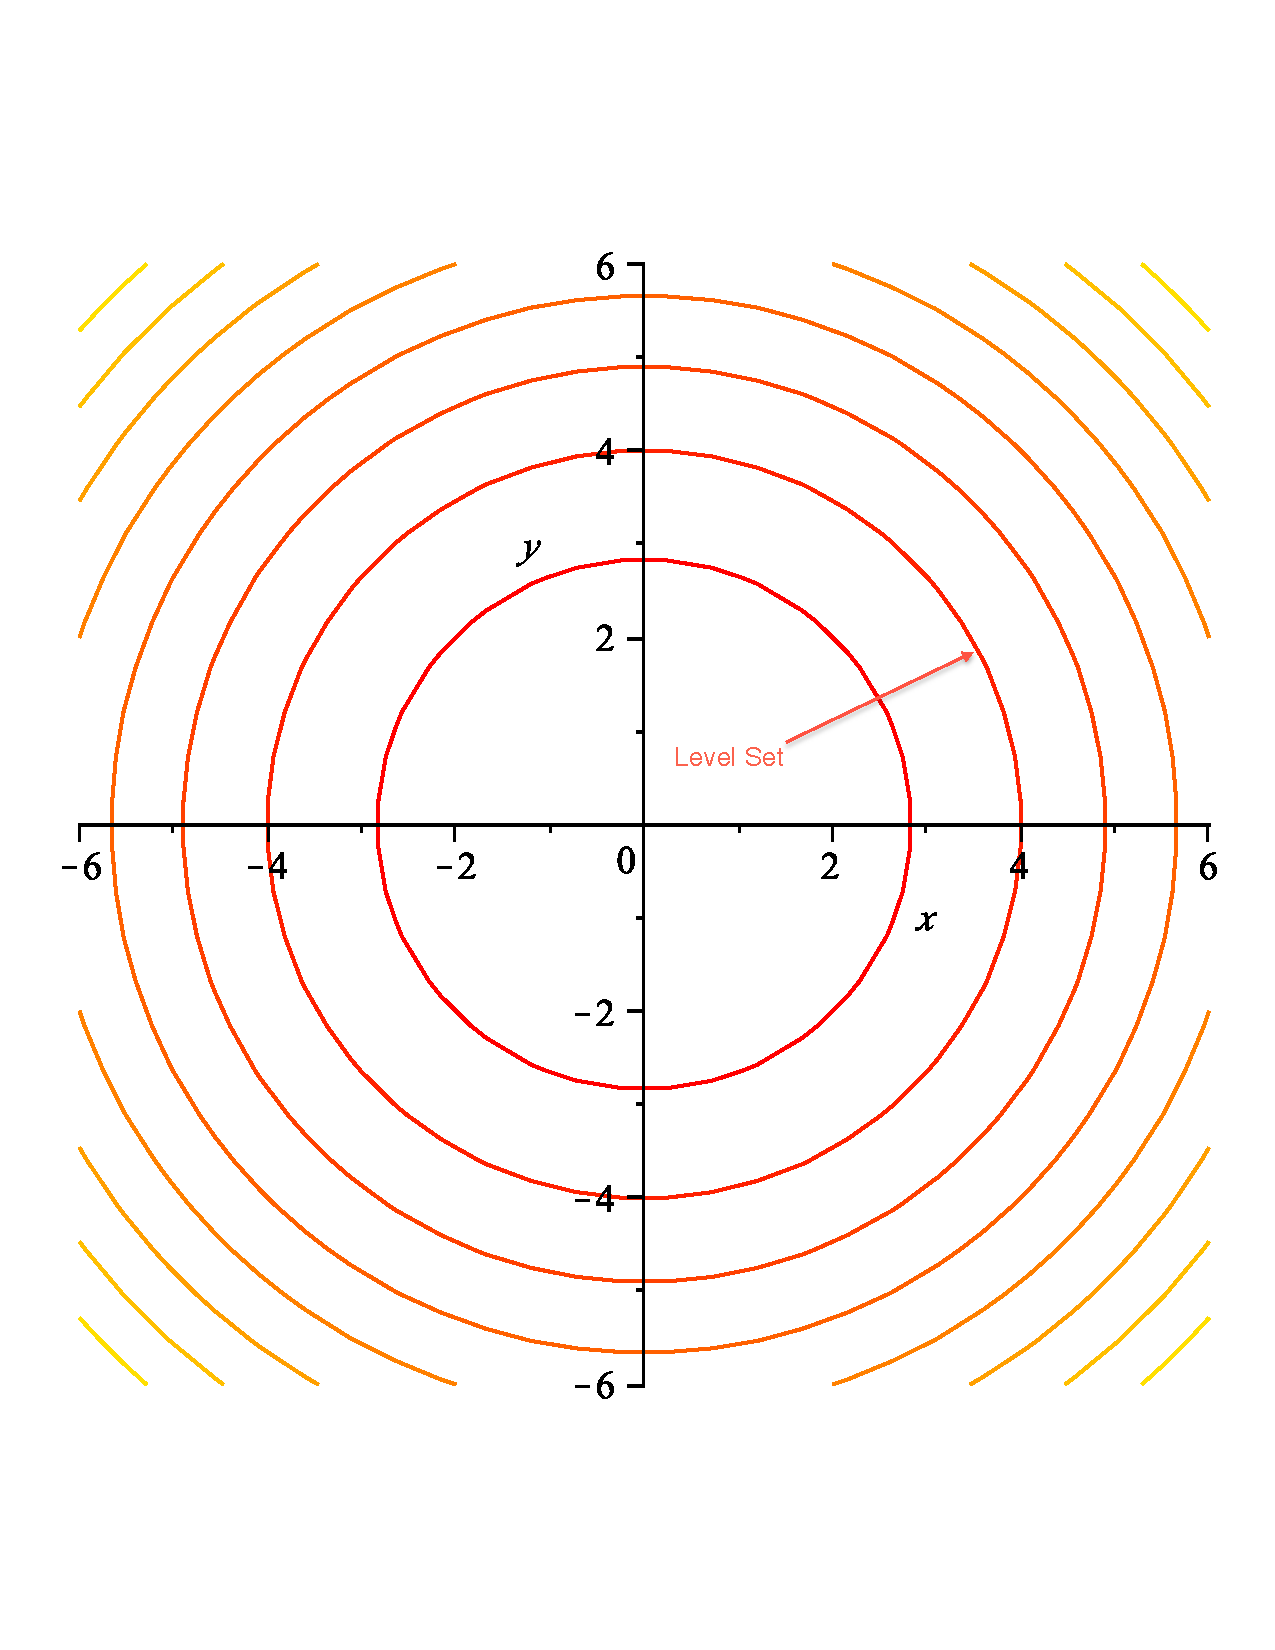
\includegraphics[scale=0.25]{ContourPlotNote.pdf}
\caption{Contour Plot of $z=x^2 + y^2$. The circles in $\mathbb{R}^2$ are the level sets of the function. The lighter the circle hue, the higher the value of $c$ that defines the level set.}
\label{fig:LevelSet2D}
\end{figure}
\label{ex:LevelSet}
\end{example}

\begin{definition}(Line) Let $\mathbf{x}_0,\mathbf{v} \in \mathbb{R}^n$. Then the \textit{line} defined by vectors $\mathbf{x}_0$ and $\mathbf{v}$ is the function $\mathbf{l}(t) = \mathbf{x}_0 + t\mathbf{v}$. Clearly $l : \mathbb{R} \rightarrow \mathbb{R}^n$. The vector $\mathbf{v}$ is called the direction of the line. 
\label{def:Line}
\end{definition} 

\begin{example}
Let $\mathbf{x_0} = (2,1)$ and let $\mathbf{v} = (2,2)$. Then the line defined by $\mathbf{x}_0$ and $\mathbf{v}$ is shown in Figure \ref{fig:LineExample}. The set of points on this line is the set $L = \{(x,y) \in \mathbb{R}^2 : x = 2 + 2t, y = 1 + 2t, t \in \mathbb{R}\}$. 
\begin{figure}[ht]
\centering
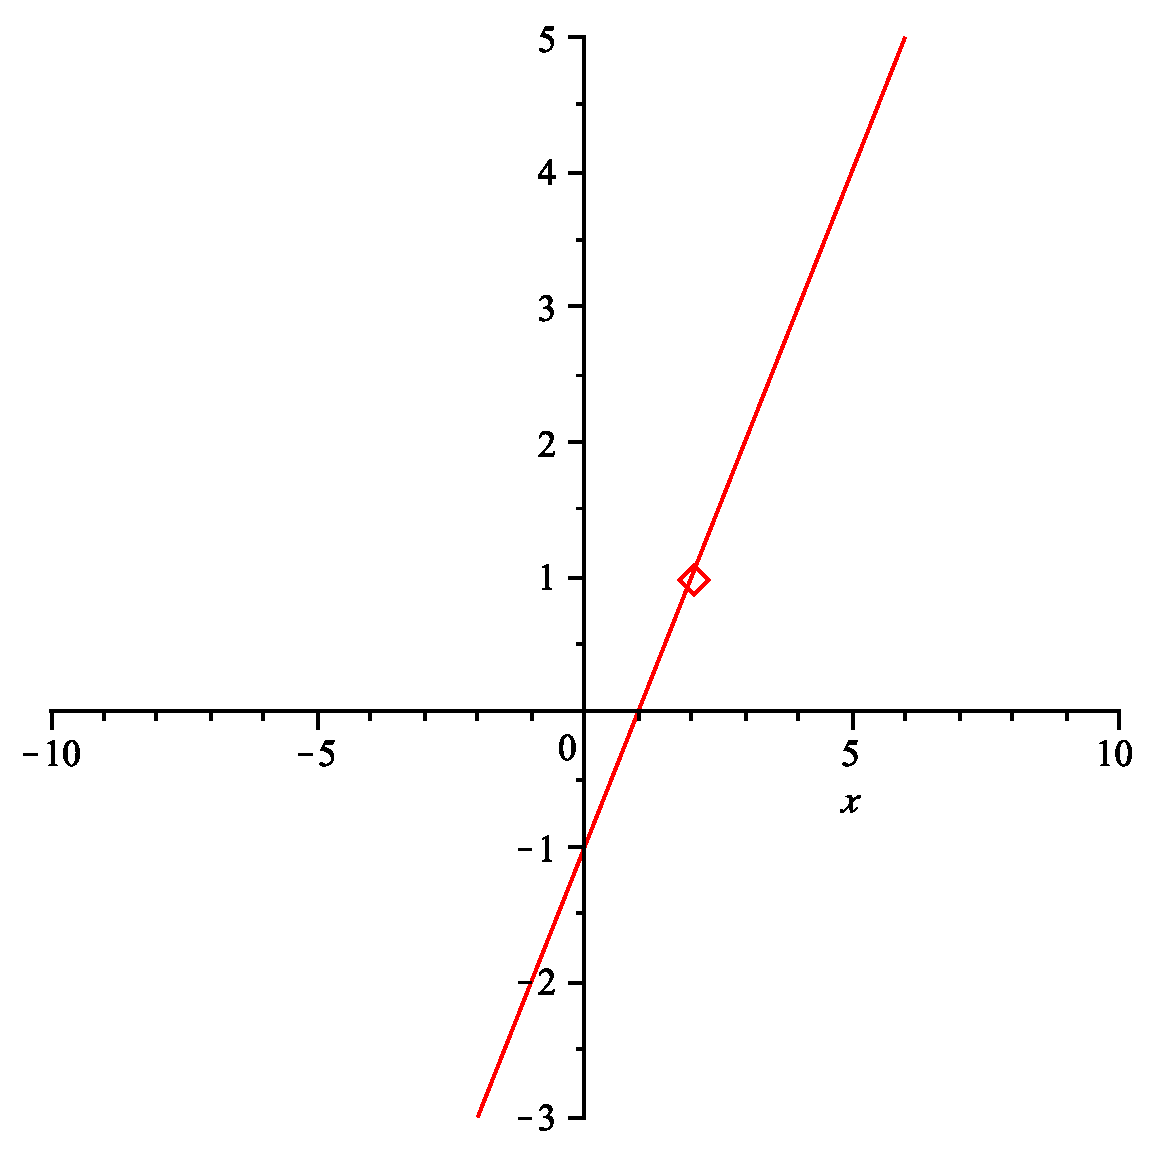
\includegraphics[scale=0.25]{LinePlot.pdf}
\caption{A Line Function: The points in the graph shown in this figure are in the set produced using the expression $\mathbf{x}_0 + \mathbf{v}t$ where $\mathbf{x_0} = (2,1)$ and let $\mathbf{v} = (2,2)$.}
\label{fig:LineExample}
\end{figure}
\label{ex:BasicLine}
\end{example}

\begin{definition}[Directional Derivative] Let $z:\mathbb{R}^n \rightarrow \mathbb{R}$ and let $\mathbf{v} \in \mathbb{R}^n$ be a vector (direction) in n-dimensional space. Then the directional derivative of $z$ at point $\mathbf{x}_0 \in\mathbb{R}^n$ in the direction of $\mathbf{v}$ is
\begin{equation}
\left.\frac{d}{dt}z(\mathbf{x}_0 + t\mathbf{v})\right\vert_{t=0}
\end{equation}
when this derivative exists.
\label{def:DirectionalDerivative}
\end{definition}

\begin{proposition} The directional derivative of $z$ at $\mathbf{x}_0$ in the direction $\mathbf{v}$ is equal to:
\begin{equation}
\lim_{h \rightarrow 0}\frac{z(\mathbf{x}_0 + h\mathbf{v}) - z(\mathbf{x}_0)}{h}
\end{equation}
\label{prop:DirecDeriv}
\end{proposition}

\begin{exercise} Prove Proposition \ref{prop:DirecDeriv}. [Hint: Use the definition of derivative for a univariate function and apply it to the definition of directional derivative and evaluate $t=0$.]
\end{exercise}
%\begin{proof} The definition of the derivative yields the expression:
%\begin{equation}
%\frac{d}{dt}z(\mathbf{x}_0 + t\mathbf{v}) = 
%\lim_{h \rightarrow 0}\frac{z(\mathbf{x}_0 + (t+h)\mathbf{v}) - z(\mathbf{x}_0 + t\mathbf{v})}{h},
%\end{equation}
%assuming that the limit exists. Evaluating the left and right hand sides at $t = 0$ yields:
%\begin{equation}
%\left.\frac{d}{dt}z(\mathbf{x}_0 + t\mathbf{v})\right\vert_{t=0} = 
%\lim_{h \rightarrow 0}\frac{z(\mathbf{x}_0 + h\mathbf{v}) - z(\mathbf{x}_0)}{h}
%\end{equation}
%This completes the proof.
%\end{proof}

\begin{definition}[Gradient]
Let $z:\mathbb{R}^n \rightarrow \mathbb{R}$ be a function and let $\mathbf{x}_0 \in \mathbb{R}^n$. Then the \textit{gradient} of $z$ at $\mathbf{x}_0$ is the vector in $\mathbb{R}^n$ given by:
\begin{equation}
\nabla z(\mathbf{x}_0) = \left(\frac{\partial z}{\partial x_1}(\mathbf{x}_0),\dots, \frac{\partial z}{\partial x_n}(\mathbf{x}_0)\right)
\end{equation}
\label{def:Gradient}
\end{definition}

Gradients are extremely important concepts in optimization (and vector calculus in general). Gradients have many useful properties that can be exploited. The relationship between the directional derivative and the gradient is of critical importance.

\begin{theorem} If $z:\mathbb{R}^n \rightarrow \mathbb{R}$ is differentiable, then all directional derivatives exist. Furthermore, the directional derivative of $z$ at $\mathbf{x}_0$ in the direction of $\mathbf{v}$ is given by:
\begin{equation}
\nabla z(\mathbf{x}_0) \cdot \mathbf{v}
\end{equation}
where $\cdot$ denotes the \textit{dot} product of two vectors.
\end{theorem}
\begin{proof} Let $\mathbf{l}(t) = \mathbf{x}_0 + \mathbf{v}t$. Then $\mathbf{l}(t) = (l_1(t),\dots,l_n(t))$; that is, $\mathbf{l}(t)$ is a vector function whose $i^{\text{th}}$ component is given by $l_i(t) = \mathbf{x}_{0_i} + \mathbf{v}_it$. 

Apply the chain rule:
\begin{equation}
\frac{dz(\mathbf{l}(t))}{dt} = 
	\frac{\partial z}{\partial l_1}\frac{dl_1}{dt} + \dots + 
	\frac{\partial z}{\partial l_n}\frac{dl_n}{dt}
\end{equation}
Thus:
\begin{equation}
\frac{d}{dt}z(\mathbf{l}(t)) = \nabla z\cdot\frac{d\mathbf{l}}{dt}
\end{equation}
Clearly $d\mathbf{l}/dt = \mathbf{v}$. We have $\mathbf{l}(0) = \mathbf{x}_0$. Thus:
\begin{equation}
\left.\frac{d}{dt}z(\mathbf{x}_0 + t\mathbf{v})\right\vert_{t=0} = 
	\nabla z(\mathbf{x}_0) \cdot \mathbf{v}
\end{equation}
\end{proof}

We now come to the two most important results about gradients, (i) the fact that they always point in the direction of steepest ascent with respect to the level curves of a function and (ii) that they are perpendicular (normal) to the level curves of a function. We can exploit this fact as we seek to maximize (or minimize) functions.

\begin{theorem} Let $z:\mathbb{R}^n \rightarrow \mathbb{R}$ be differentiable, $\mathbf{x}_0 \in \mathbb{R}^n$. If $\nabla z(\mathbf{x}_0) \neq 0$, then $\nabla z(\mathbf{x}_0)$ points in the direction in which $z$ is increasing fastest.
\end{theorem}
\begin{proof} Recall $\nabla z(\mathbf{x}_0)\cdot \mathbf{v}$ is the directional derivative of $z$ in direction $\mathbf{v}$ at $\mathbf{x}_0$. Assume that $\mathbf{v}$ is a unit vector. We know that:
\begin{equation}
\nabla z(\mathbf{x}_0)\cdot \mathbf{v}  = ||\nabla z(\mathbf{x}_0)||\cos\theta
\end{equation}
(because we assumed $\mathbf{v}$ was a unit vector) where $\theta$ is the angle between the vectors $\nabla z(\mathbf{x}_0)$ and $\mathbf{v}$. The function $\cos\theta$ is largest when $\theta = 0$, that is when $\mathbf{v}$ and $\nabla z(\mathbf{x}_0)$ are parallel vectors. (If $\nabla z(\mathbf{x}_0) = 0$, then the directional derivative is zero in all directions.)
\end{proof}

\begin{theorem} Let $z:\mathbb{R}^n \rightarrow \mathbb{R}$ be differentiable and let $\mathbf{x}_0$ lie in the level set $S$ defined by $z(\mathbf{x}) = k$ for fixed $k \in \mathbb{R}$. Then $\nabla z(\mathbf{x}_0)$ is normal to the set $S$ in the sense that if $\mathbf{v}$ is a tangent vector at $t = 0$ of a path $\mathbf{c}(t)$ contained entirely in $S$ with $\mathbf{c}(0) = \mathbf{x}_0$, then $\nabla z(\mathbf{x}_0) \cdot \mathbf{v} = 0$. 
\label{thm:GradPerpLevelSet}
\end{theorem}

\begin{remark} Before giving the proof, we illustrate this theorem in Figure \ref{fig:LevelSetWithVector}. The function is $z(x,y) = x^4+y^2+2xy$ and $\mathbf{x}_0 = (1,1)$. At this point $\nabla z(\mathbf{x}_0) = (6,4)$. We include the tangent line to the level set at the point (1,1) to illustrate the normality of the gradient to the level curve at the point.
\end{remark}

\begin{figure}[htbp]
\centering
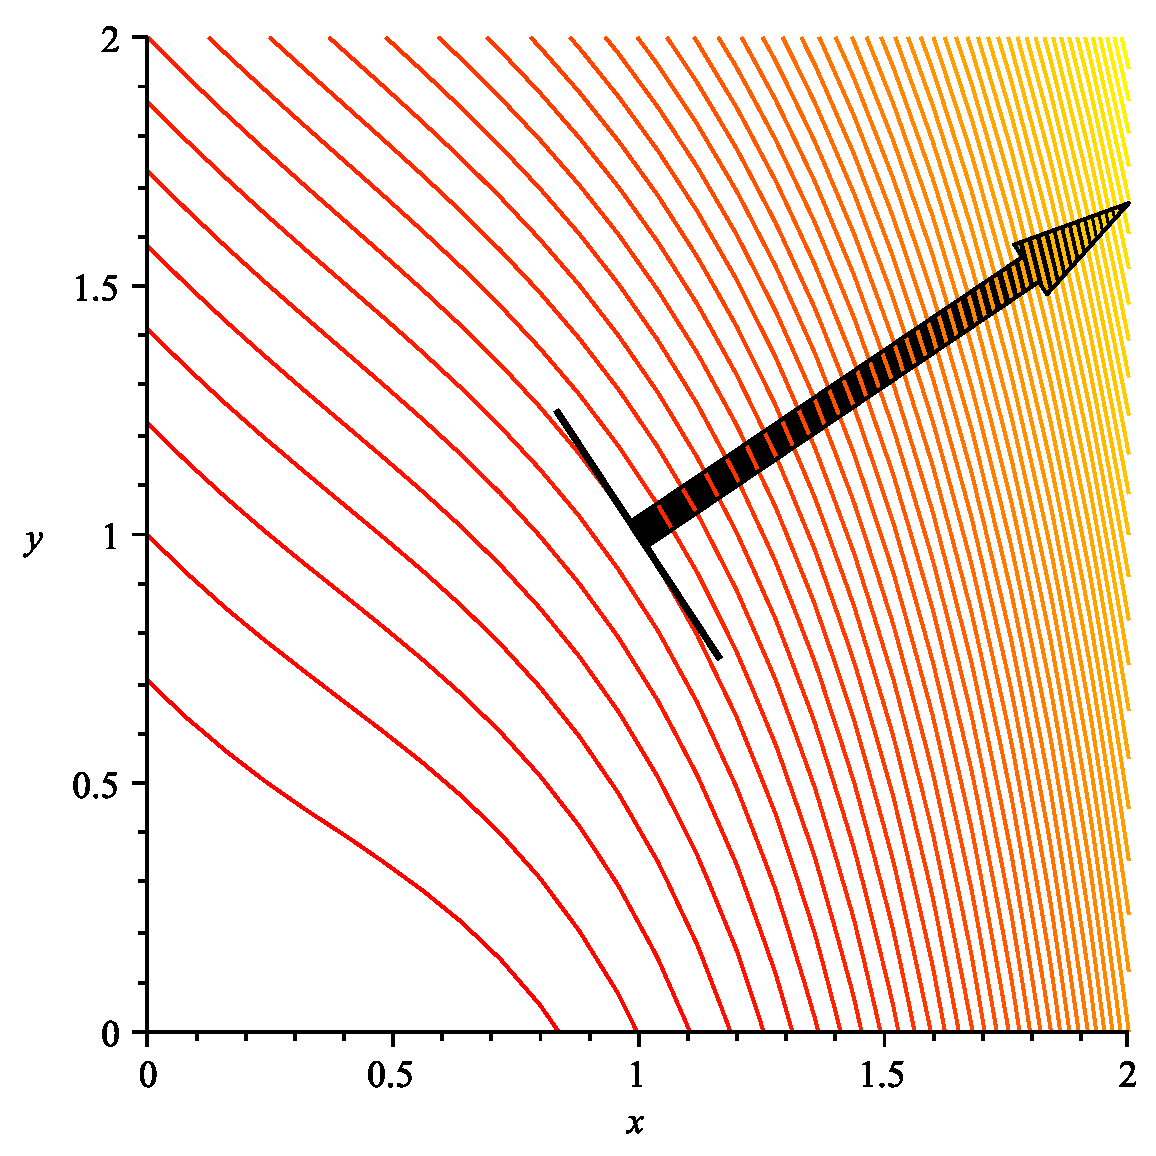
\includegraphics[scale=0.35]{LevelSetsWithVector.pdf}
\caption{A Level Curve Plot with Gradient Vector: We've scaled the gradient vector in this case to make the picture understandable. Note that the gradient is perpendicular to the level set curve at the point $(1,1)$, where the gradient was evaluated. You can also note that the gradient is pointing in the direction of steepest ascent of $z(x,y)$.}
\label{fig:LevelSetWithVector}
\end{figure}

\begin{proof} As stated, let $\mathbf{c}(t)$ be a curve in $S$. Then $\mathbf{c}:\mathbb{R} \rightarrow \mathbb{R}^n$ and $z(\mathbf{c}(t) ) = k$ for all $t \in \mathbb{R}$. Let $\mathbf{v}$ be the tangent vector to $\mathbf{c}$ at $t = 0$; that is:
\begin{equation}
\left.\frac{d\mathbf{c}(t)}{dt}\right|_{t=0} = \mathbf{v}
\end{equation}
Differentiating $z(\mathbf{c}(t))$ with respect to $t$ using the chain rule and evaluating at $t = 0$ yields:
\begin{equation}
\left.\frac{d}{dt}z(\mathbf{c}(t))\right|_{t=0} = \nabla z(\mathbf{c}(0))\cdot\mathbf{v} = \nabla z(\mathbf{x}_0) \cdot \mathbf{v} = 0
\end{equation}
Thus $\nabla z(\mathbf{x}_0)$ is perpendicular to $\mathbf{v}$ and thus normal to the set $S$ as required.
\end{proof}

\begin{remark}There's a simpler proof of this theorem in the case of a mapping $z : \mathbb{R}^2 \rightarrow \mathbb{R}$. For any such function $z(x,y)$, we know that a level set is an implicitly defined curve given by the expression
\begin{displaymath}
z(x,y) = k
\end{displaymath}
where $k \in \mathbb{R}$. We can compute the slope of any tangent line to this curve at some point $(x_0,y_0)$ with implicit differentiation. We have:
\begin{displaymath}
\left(\frac{d}{dx}\right) z(x,y) = k \left(\frac{d}{dx}\right)
\end{displaymath}
yields:
\begin{displaymath}
\frac{\partial z}{\partial x} + \frac{\partial z}{\partial y}\frac{dy}{dx}  = 0 
\end{displaymath}
Then the slope of the tangent line is given by:
\begin{displaymath}
\frac{dy}{dx} = \frac{-\partial z/\partial x}{\partial z/\partial y}
\end{displaymath}
By $z_x(x_0,y_0)$ we mean $\partial z/\partial x$ evaluated at $(x_0,y_0)$ and by $z_y(x_0,y_0)$ we mean $\partial z/\partial y$ evaluated at $(x_0,y_0)$. Then the slope of the tangent line to the curve $z(x,y) = k$ at $(x_0,y_0)$ is:
\begin{displaymath}
m = \frac{-z_x(x_0,y_0)}{z_y(x_0,y_0)}
\end{displaymath}
An equation for the tangent line at this point is:
\begin{equation}
y - y_0 = m(x - x_0)
\label{eqn:PointSlope}
\end{equation}
We can compute a vector that is parallel to this line by taking two points on the line, $(x_0,y_0)$ and $(x_1, y_1)$ and computing the vector $(x_1 - x_0, y_1 - y_0)$. We know that:
\begin{displaymath}
y_1 - y_0 = m(x_1 - x_0)
\end{displaymath}
because any pair $(x_1,y_1)$ on the tangent line must satisfy Equation \ref{eqn:PointSlope}. Thus we have the vector $\mathbf{v} = (x_1 - x_0, m(x_1 - x_0))$ parallel to the tangent line. Now we compute the dot product of this vector with the gradient of the function:
\begin{displaymath}
\nabla z(x_0,y_0) = (z_x(x_0,y_0), z_y(x_0,y_0))
\end{displaymath}
We obtain:
\begin{multline*}
\nabla z(x_0,y_0)\cdot\mathbf{v} = z_x(x_0,y_0)\left(x_1 - x_0\right) + z_y(x_0,y_0)\left(m(x_1 - x_0)\right) = \\z_x(x_0,y_0)\left(x_1 - x_0\right) + 
z_y(x_0,y_0)\left(\frac{-z_x(x_0,y_0)}{z_y(x_0,y_0)}(x_1 - x_0)\right)
 = \\
z_x(x_0,y_0)\left(x_1 - x_0\right) + \left(-z_x(x_0,y_0)(x_1 - x_0)\right) = 0
\end{multline*}
Thus, $\nabla z(x_0,y_0)$ is perpendicular to $\mathbf{v}$ as we expected from Theorem \ref{thm:GradPerpLevelSet}
\end{remark}

\begin{example} Let's demonstrate the previous remark and Theorem \ref{thm:GradPerpLevelSet}. Consider the function $z(x,y) = x^4 + y^2 + 2xy$ with a point $(x_0,y_0)$. Any level curve of the function is given by: $x^4 + y^2 + 2xy = k$. Taking the implicit derivative we obtain:
\begin{displaymath}
\left(\frac{d}{dx}\right)x^4 + y^2 + 2xy = k\left(\frac{d}{dx}\right) \implies 
4x^3 + 2y\frac{dy}{dx} + 2y + 2x\frac{dy}{dx} = 0
\end{displaymath}
Note that to properly differentiate $2xy$ implicitly, we needed to use the product rule from calculus. Now, we can solve for the slope of the tangent line to the curve at point $(x_0,y_0)$ as:
\begin{displaymath}
m = \left(\frac{dy}{dx}\right) = \frac{-4x_0^3 - 2y_0}{2y_0 + 2x_0}
\end{displaymath}
Our tangent line is then described the equation:
\begin{displaymath}
y - y_0 = m(x - x_0)
\end{displaymath}
Using the same reasoning we did in the remark, a vector parallel to this line is given by $(x_1 - x_0, y_1 - y_0)$ where $(x_1, y_1)$ is another point on the tangent line. Then we know that:
\begin{displaymath}
y_1 - y_0 = m(x_1 - x_0)
\end{displaymath}
and thus our vector is $\mathbf{v} = (x_1 - x_0, m(x_1 - x_0))$. Now, computing the gradient of $z(x,y)$ at $(x_0,y_0)$ is:
\begin{displaymath}
\nabla z(x_0,y_0) = (4x_0^3 + 2y_0, 2y_0 + 2x_0)
\end{displaymath} 
Lastly we compute:
\begin{multline*}
\nabla z(x_0,y_0)\cdot\mathbf{v} = \left(4x_0^3 + 2y_0\right)(x_1 - x_0) + 
\left(2y_0 + 2x_0\right)\left(m(x_1 - x_0)\right) = \\
\left(4x_0^3 + 2y_0\right)(x_1 - x_0) + \left(2y_0 + 2x_0\right)\left(\frac{-4x_0^3 - 2y_0}{2y_0 + 2x_0}(x_1 - x_0)\right) = \\
\left(4x_0^3 + 2y_0\right)(x_1 - x_0) + \left(-4x_0^3 - 2y_0\right)(x_1 - x_0) = 0
\end{multline*}
Thus, for any point $(x_0,y_0)$ on a level curve of $z(x,y) = x^4 + y^2 + 2xy$ we know that the gradient at that point is perpendicular to a tangent line (vector) to the curve at the point $(x_0,y_0)$. 

It is interesting to note that one can compute the slope of the tangent line (and its equation) in Figure \ref{fig:LevelSetWithVector}. Here $(x_0,y_0) = (1,1)$, thus the slope of the tangent line is:
\begin{displaymath}
m = \frac{-4x_0^3 - 2y_0}{2y_0 + 2x_0} = \frac{-6}{4} = \frac{-3}{2}
\end{displaymath}
The equation for the line displayed in Figure \ref{fig:LevelSetWithVector} is:
\begin{displaymath}
y - 1 = \frac{-3}{2}(x - 1)
\end{displaymath}
\end{example}

\begin{exercise} In this exercise you will use elementary calculus (and a little bit of vector algebra) to show that the gradient of a simple function is perpendicular to its level sets:
\begin{description*}
\item[(a)] Plot the level sets of $z(x,y) = x^2 + y^2$. Draw the gradient at the point $(x,y) = (2,0)$. Convince yourself that it is normal to the level set $x^2 + y^2 = 4$. 

\item[(b)] Now, choose any level set $x^2 + y^2 = k$. Use implicit differentiation to find $dy/dx$. This is the slope of a tangent line to the circle $x^2 + y^2 = k$. Let $(x_0,y_0)$ be a point on this circle.

\item[(c)] Find an expression for a vector parallel to the tangent line at $(x_0,y_0)$ [Hint: you can use the slope you just found.] 

\item[(d)] Compute the gradient of $z$ at $(x_0,y_0)$ and use it and the vector expression you just computed to show that two vectors are perpendicular. [Hint: use the dot product.]
\end{description*}
\end{exercise} 

\section{Gradients, Constraints and Optimization}
Since we're talking about optimization (i.e., minimizing or maximizing a certain function subject to some constraints), it follows that we should be interested in the gradient, which indicates the direction of greatest increase in a function. This information will be used in maximizing a function. Logically, the negation of the gradient will point in the direction of greatest decrease and can be used in minimization. We'll formalize these notions in the study of linear programming. We make one more definition:

\begin{definition}[Binding Constraint] Let $g(\mathbf{x}) \leq b$ be a constraint in an optimization problem. If at point $\mathbf{x}_0 \in \mathbb{R}^n$ we have $g(\mathbf{x}_0) = b$, then the constraint is said to be \textit{binding}. Clearly equality constraints $h(\mathbf{x}) = r$ are always binding.
\end{definition}

\begin{example}[Continuation of Example \ref{ex:GoatExample}] Let's look at the level curves of the objective function and their relationship to the constraints at the point of optimality $(x,y) = (25,25)$. In Figure \ref{fig:Goat2DPlot} we see the level curves of the objective function (the hyperbolas) and the feasible region shown as shaded. The elements in the feasible regions are all values for $x$ and $y$ for which $2x + 2y \leq 100$ and $x,y \geq 0$. You'll note that at the point of optimality the level curve $xy = 625$ is tangent to the equation $2x + 2y = 100$; i.e., the level curve of the objective function is tangent to the binding constraint.
\begin{figure}[htbp]
\centering
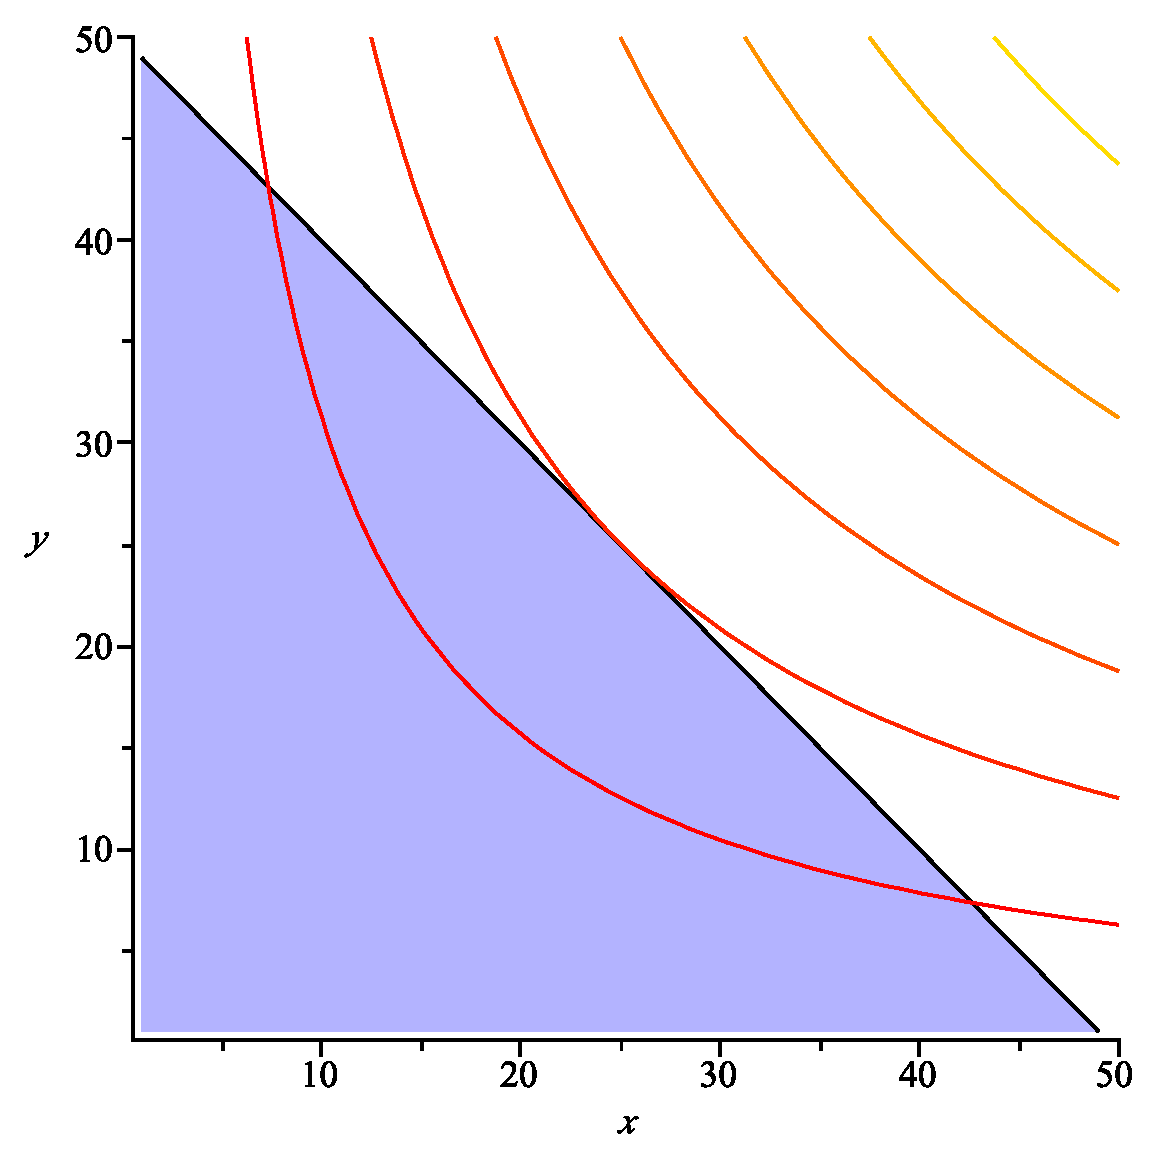
\includegraphics[scale=0.35]{GoatConstraintObjective.pdf}
\caption{Level Curves and Feasible Region: At optimality the level curve of the objective function is tangent to the binding constraints.}
\label{fig:Goat2DPlot}
\end{figure}

If you look at the gradient of $A(x,y)$ at this point it has value $(25,25)$. We see that it is pointing in the direction of increase for the function $A(x,y)$ (as should be expected) but more importantly let's look at the gradient of the function $2x + 2y$. It's gradient is $(2,2)$, which is just a scaled version of the gradient of the objective function. Thus the gradient of the objective function is just a dilation of gradient of the binding constraint. This is illustrated in Figure \ref{fig:Goat2DPlotWithGrad}.
\begin{figure}[htbp]
\centering
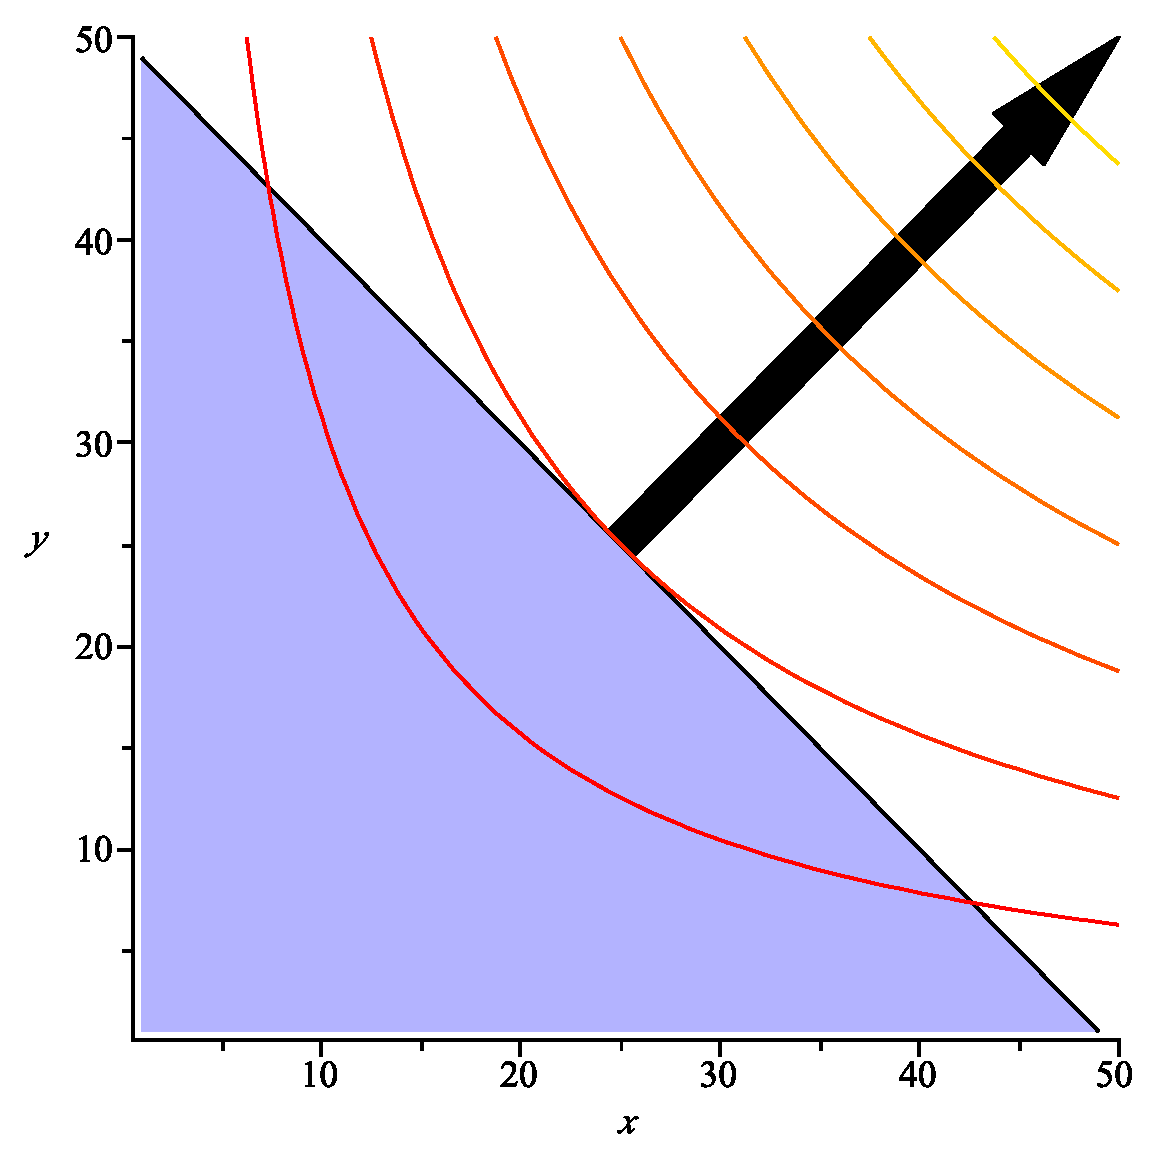
\includegraphics[scale=0.35]{GoatConstraintObjectiveWithGrad.pdf}
\caption{Gradients of the Binding Constraint and Objective: At optimality the gradient of the binding constraints and the objective function are \textit{scaled versions of each other}.}
\label{fig:Goat2DPlotWithGrad}
\end{figure}
\end{example}

The elements illustrated in the previous example are true in general. You may have discussed a simple example of these when you talked about \textit{Lagrange Multipliers} in Vector Calculus (Math 230/231). We'll revisit these concepts later when we talk about \textit{duality theory} for linear programs. We'll also discuss the gradients of the binding constraints with respect to optimality when we discuss linear programming. 

\begin{exercise} Plot the level sets of the objective function and the feasible region in Exercise \ref{exer:Can}. At the point of optimality you identified, show that the gradient of the objective function is a scaled version of the gradient (linear combination) of the binding constraints.
\end{exercise}
